\section{Chemical Protective Clothing and Its Applications}
\label{sec:CPC}

Scenarios where workers are exposed to hazardous materials require chemical protective clothing (CPC). Protection levels range from limited spray protection (Type 6) to fully encapsulating, gas-tight suits (Type 1) with self-contained breathing apparatus (SCBA)\footnote{A self-contained breathing apparatus consists of a respirator connected to a gas cylinder supplying breathable air. The cylinder is fastened to a harness worn on the back.} [\citetitle{DGUVInformation212019}].

\begin{figure}[hbt]
    \centering
    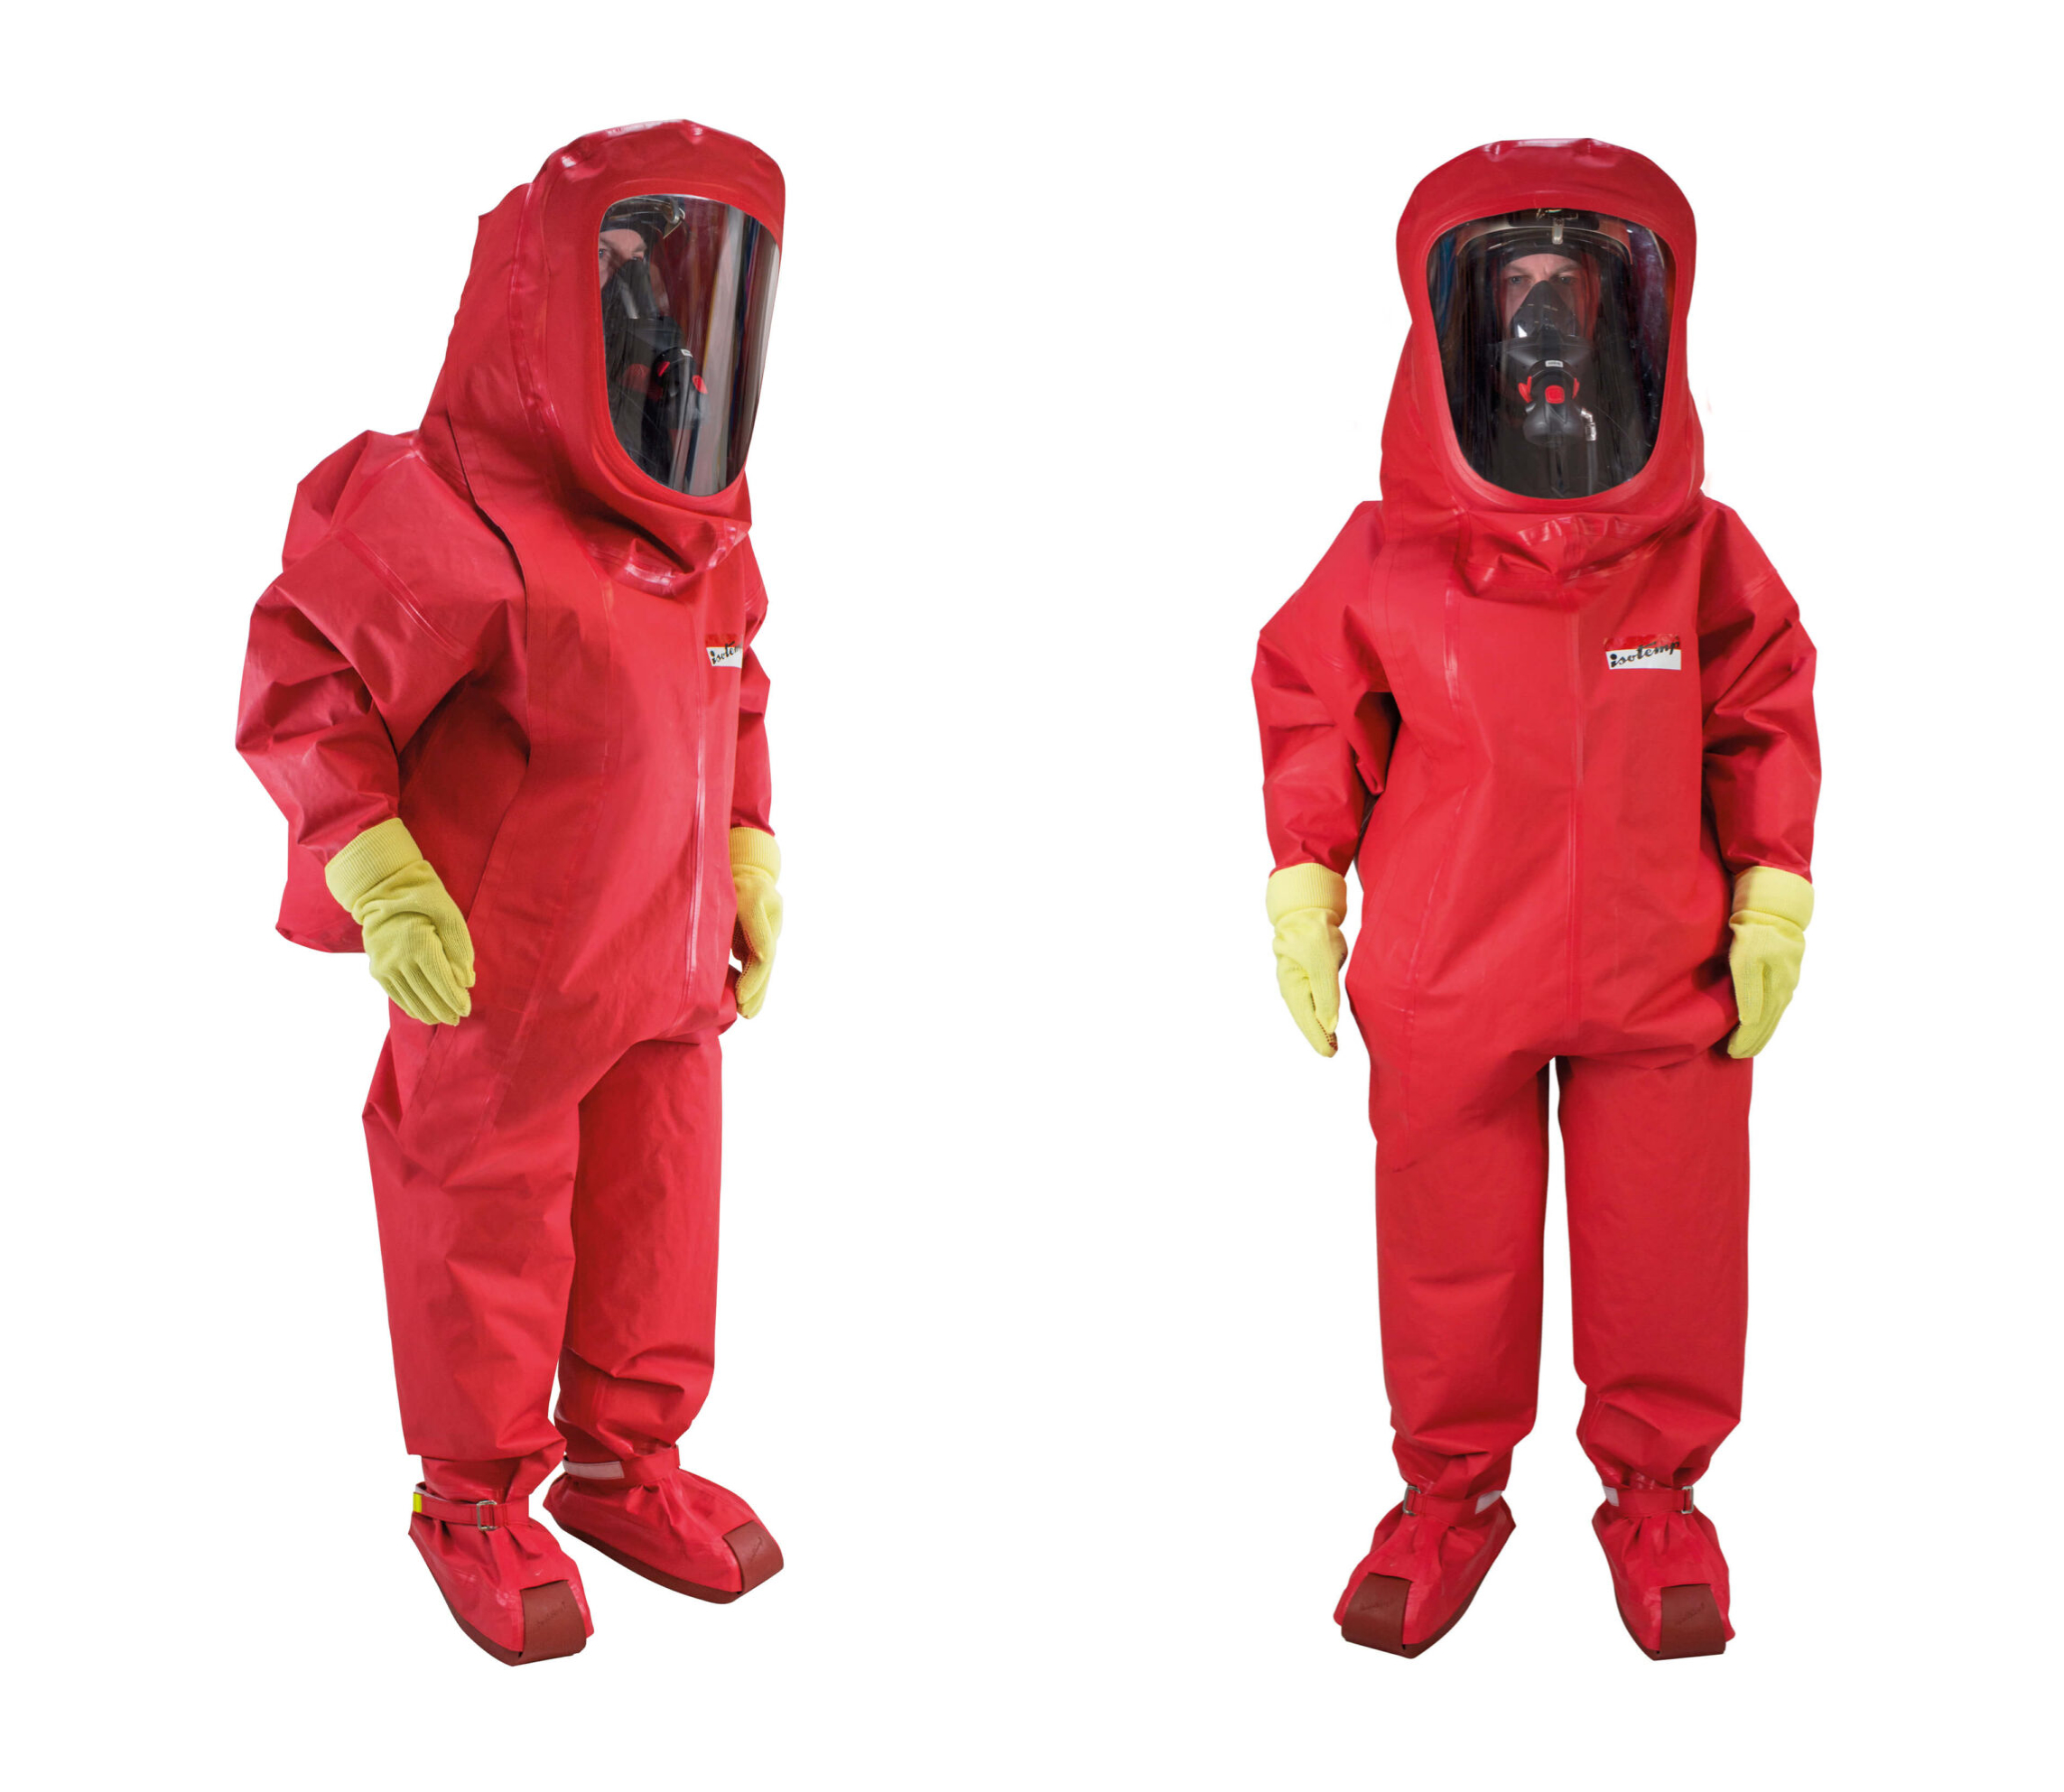
\includegraphics[width=0.8\textwidth]{assets/CPC_isotemp.jpg}
    \captionbelow[Chemical protection suit 4005/NEO manufactured by isotemp]{Type 1 chemical protection suit 4005/NEO manufactured by isotemp\protect\footnotemark}
    \label{fig:CPC_isotemp}
\end{figure}

\footnotetext{\href{https://www.isotemp.de/produkte/vollschutzanzug-4005-neo/}{Vollschutzanzug 4005/NEO · Chemie · isotemp}}

Confined spaces are defined as areas in which, through their design or site conditions, "inadequate air replacement rates, or the substances [...] found within them or introduced into them, particular hazards exist or may arise that substantially exceed the normal prevailing hazard potential of workplaces" [\citetitle{DGUVRegel113004}]. Tasks that require entering confined spaces are typically cleaning, inspection and/or maintenance of, for example, tanks in chemical plants, rail cars and highway tank trailers and even sewage containers. Traces of the contents may remain, even if their containers are prepared correctly. These residues might—despite being initially inactive—become dangerous through work procedures (e.g. welding), agitation or chemical reactions [\citetitle{DGUVRegel113004}], hence requiring the highest levels of protection. Other use cases are emergencies, such as confined space rescue, removing chemical spills or other accidents involving unknown, possibly hazardous substances [\citetitle{OSHATechnicalManual}].

These tasks are highly demanding—both physically and mentally—particularly because of the equipment. Since Type 1 suits are not gas-permeable, they compromise the body's ability to regulate temperature, leading to exhaustion and heat fatigue even faster [\cite{holmerProtectiveClothingHot2006}]. The exertion is exacerbated by heavier equipment and heat stress, ultimately reducing work capacity and performance [\cite{smolanderCardiorespiratoryThermalEffects1984}]. The maximum working time in a full-body suit with SCBA is therefore limited and might decrease even more depending on oxygen and exhaustion levels.

Further, the material and shape of the suit limit mobility and the field of view to such an extent that even trained personnel may take twice as long to complete tasks when wearing CPC [\cite{murrayEffectsChemicalProtective2011}].

% The decreased vision makes it more difficult to keep track of surroundings, which is important.
% A HUD could provide relevant information to offset this restriction of senses.